
\begin{center}
	\Huge
	Differentialkvotienten
\end{center}

\stepcounter{section}

Vi har allerede defineret differentialkvotienten som hældningen af tangenten i et punkt.  Vi har dog ikke nogen præcis definition af, hvad en tangent i et punkt reelt set er. Vi vil derfor give en mere præcis definition af hældningen af tangenten. Vi tager udgangspunkt i et eksempel.

\begin{exa}
Vi forestiller os, at vi kører i en bil, og vi er interesserede i hvor stærkt, vi kører på et tidspunkt $t$. Lad os sige, at vi fra tidspunkt $t$ til tidspunkt $t+5$ måler, at vi er kørt $200m$. Så ved vi, at vi i gennemsnit har kørt med en hastighed på
\begin{align*}
\frac{200m}{5s} = 40\frac{m}{s},
\end{align*} 
men vi ved fortsat ikke, hvor stærkt vi kørte nøjagtigt ved tid $t$. Vi måler derfor, at vi til tidspunkt $t+2$ har kørt $70m$. Vi ved derfor, at vi fra tid $t$ til tid $t+2$ har kørt med en hastighed på 
\begin{align*}
\frac{70m}{2s} = 35\frac{m}{s},
\end{align*}
og vi kommer en smule nærmere den korrekte hastighed til tid $t$. Den korrekte hastighed må derfor blive tilnærmet mere og mere jo mindre tidsinterval, vi måler hen over bliver. 
\end{exa}
Inspireret af dette eksempel, vil vi definere den såkaldte differentialkvotient, der fortæller noget om den øjeblikkelige tilvækst af en funktion. 
Betragt funktionen på Fig. \ref{fig:sek1}
\begin{figure}[H]
\centering
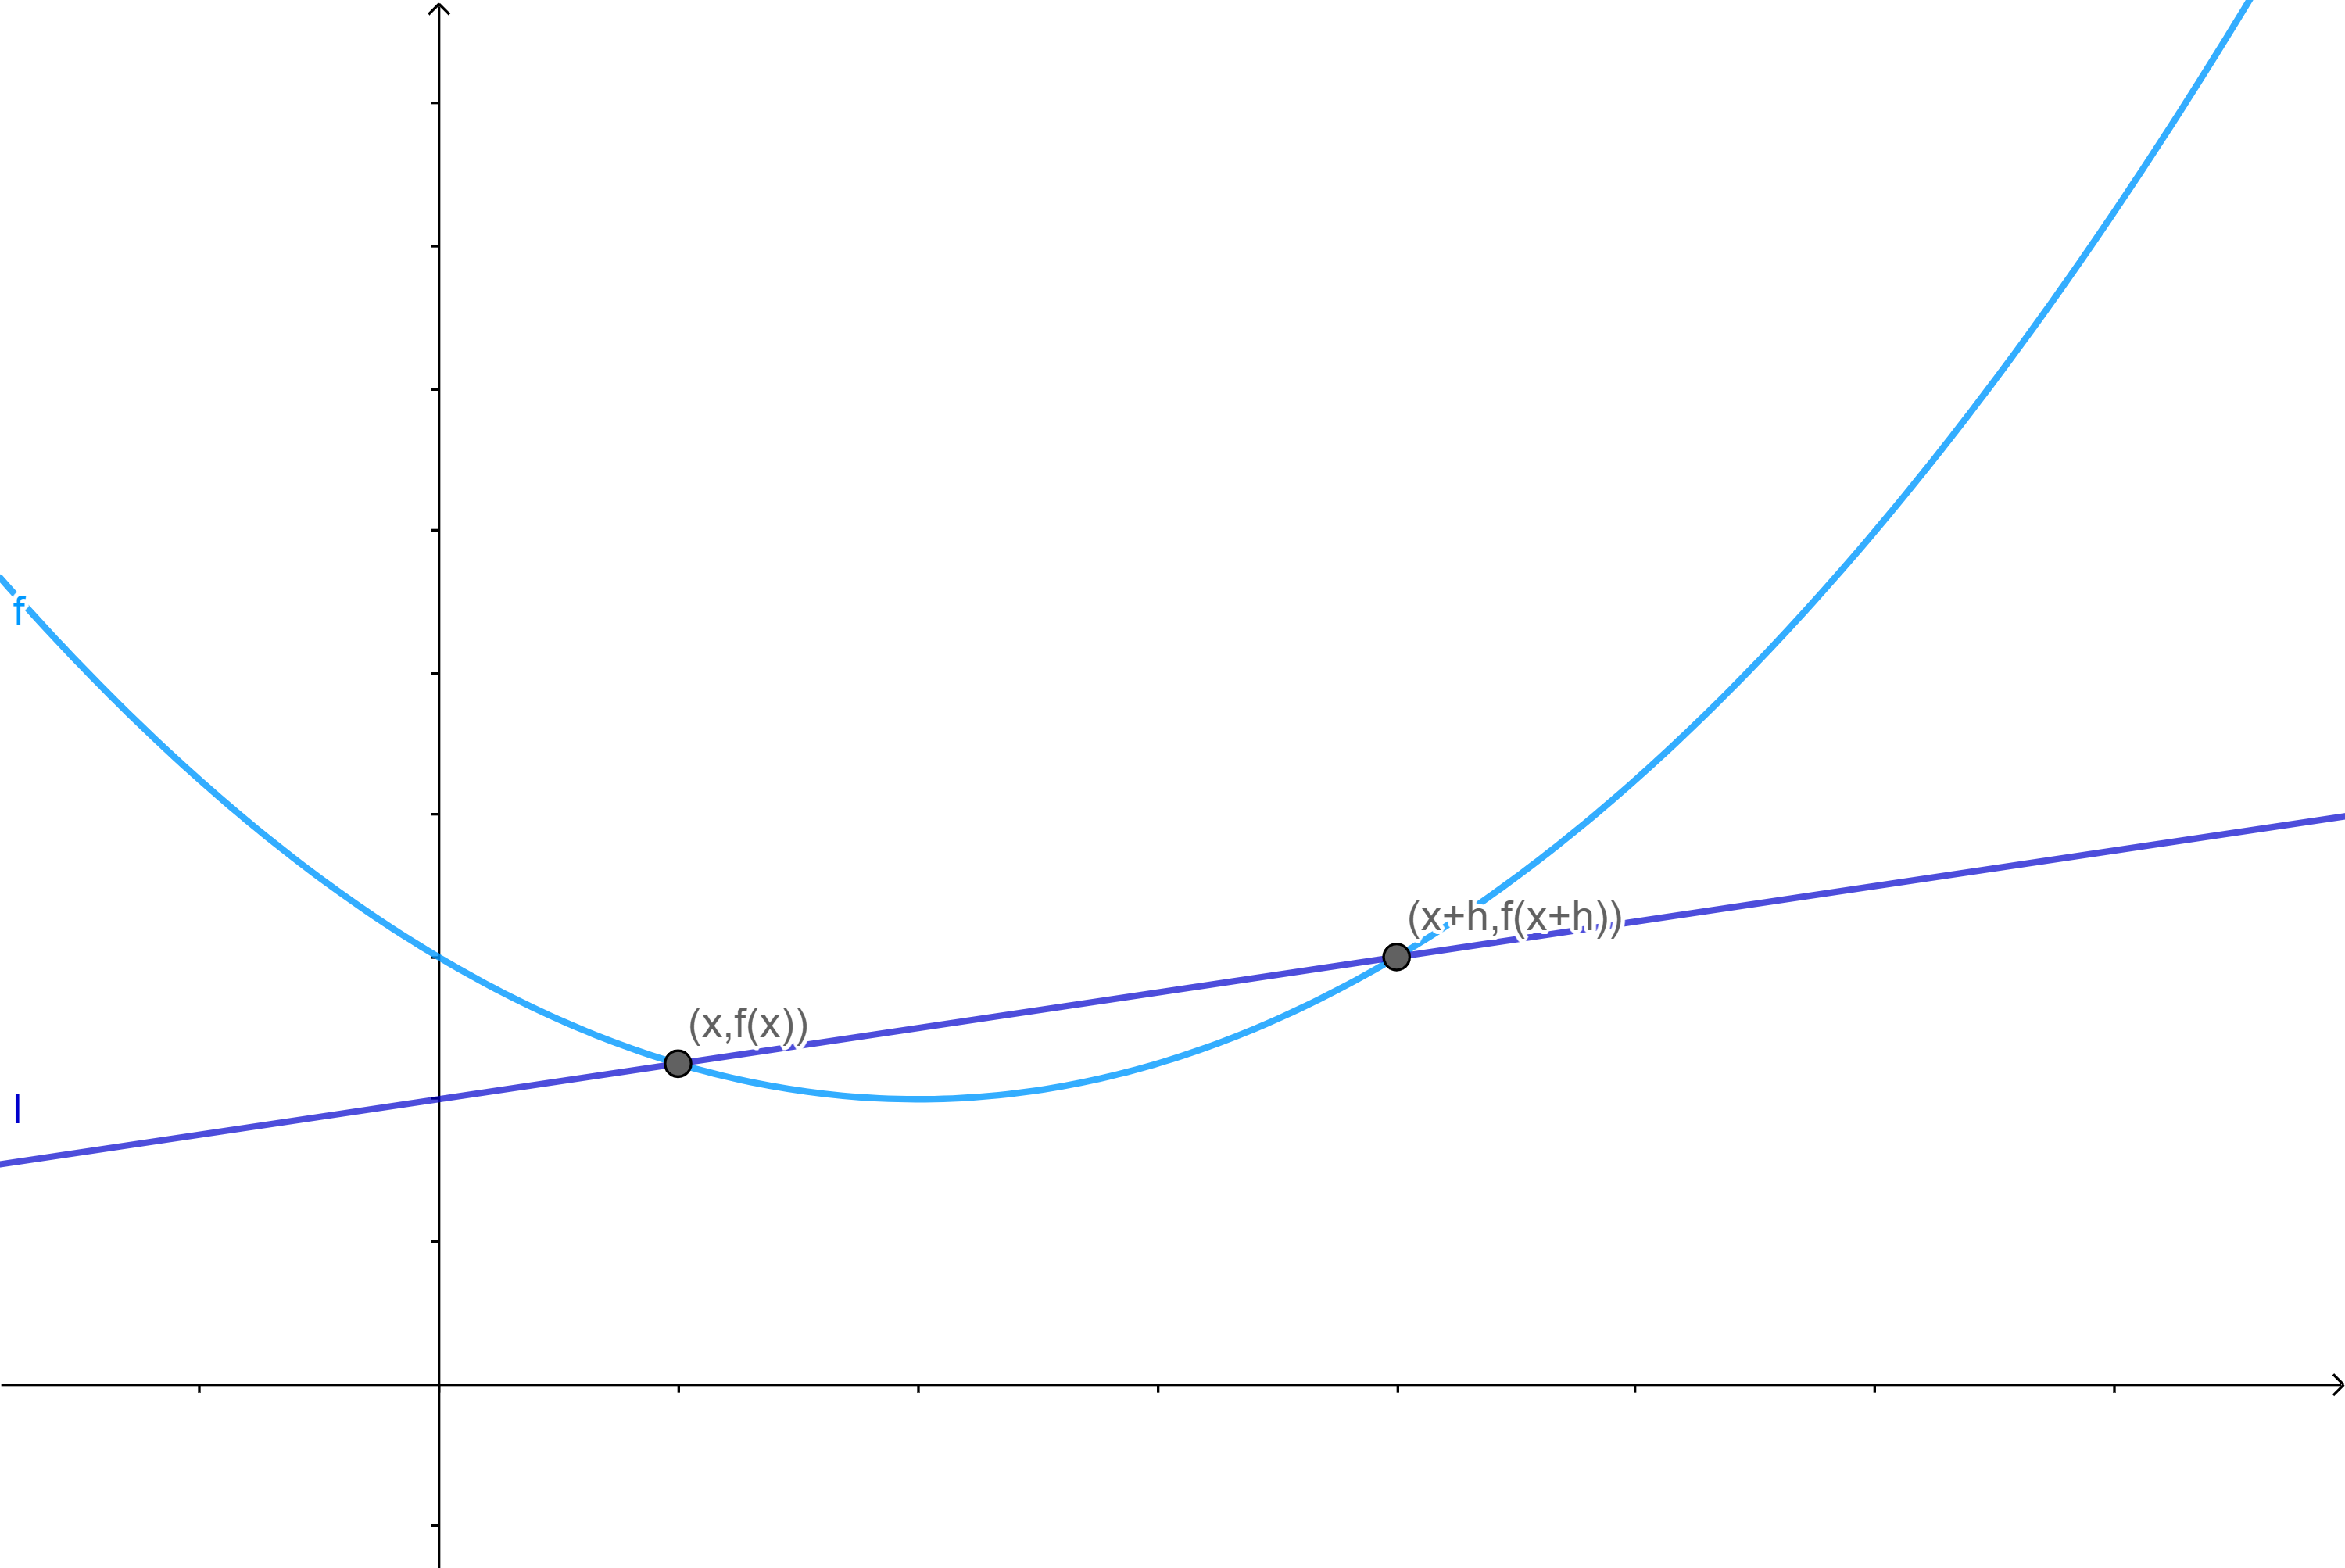
\includegraphics[width = 12cm]{Billeder/sekant1.png}
\caption{Funktion med sekant gennem punkterne $(x_0,f(x_0))$ og $(x_0+h,f(x_0+h))$.}
\label{fig:sek1}
\end{figure}
Lader vi $h$ blive mindre, så vil sekanten gennem punkterne $(x_0,f(x_0))$ og $(x_0+h,f(x_0+h))$ komme tættere og tættere på at være tangent til funktionen $f$ i punktet $(x_0,f(x_0))$, som vi ser på Figur 2.
\begin{figure}[H]
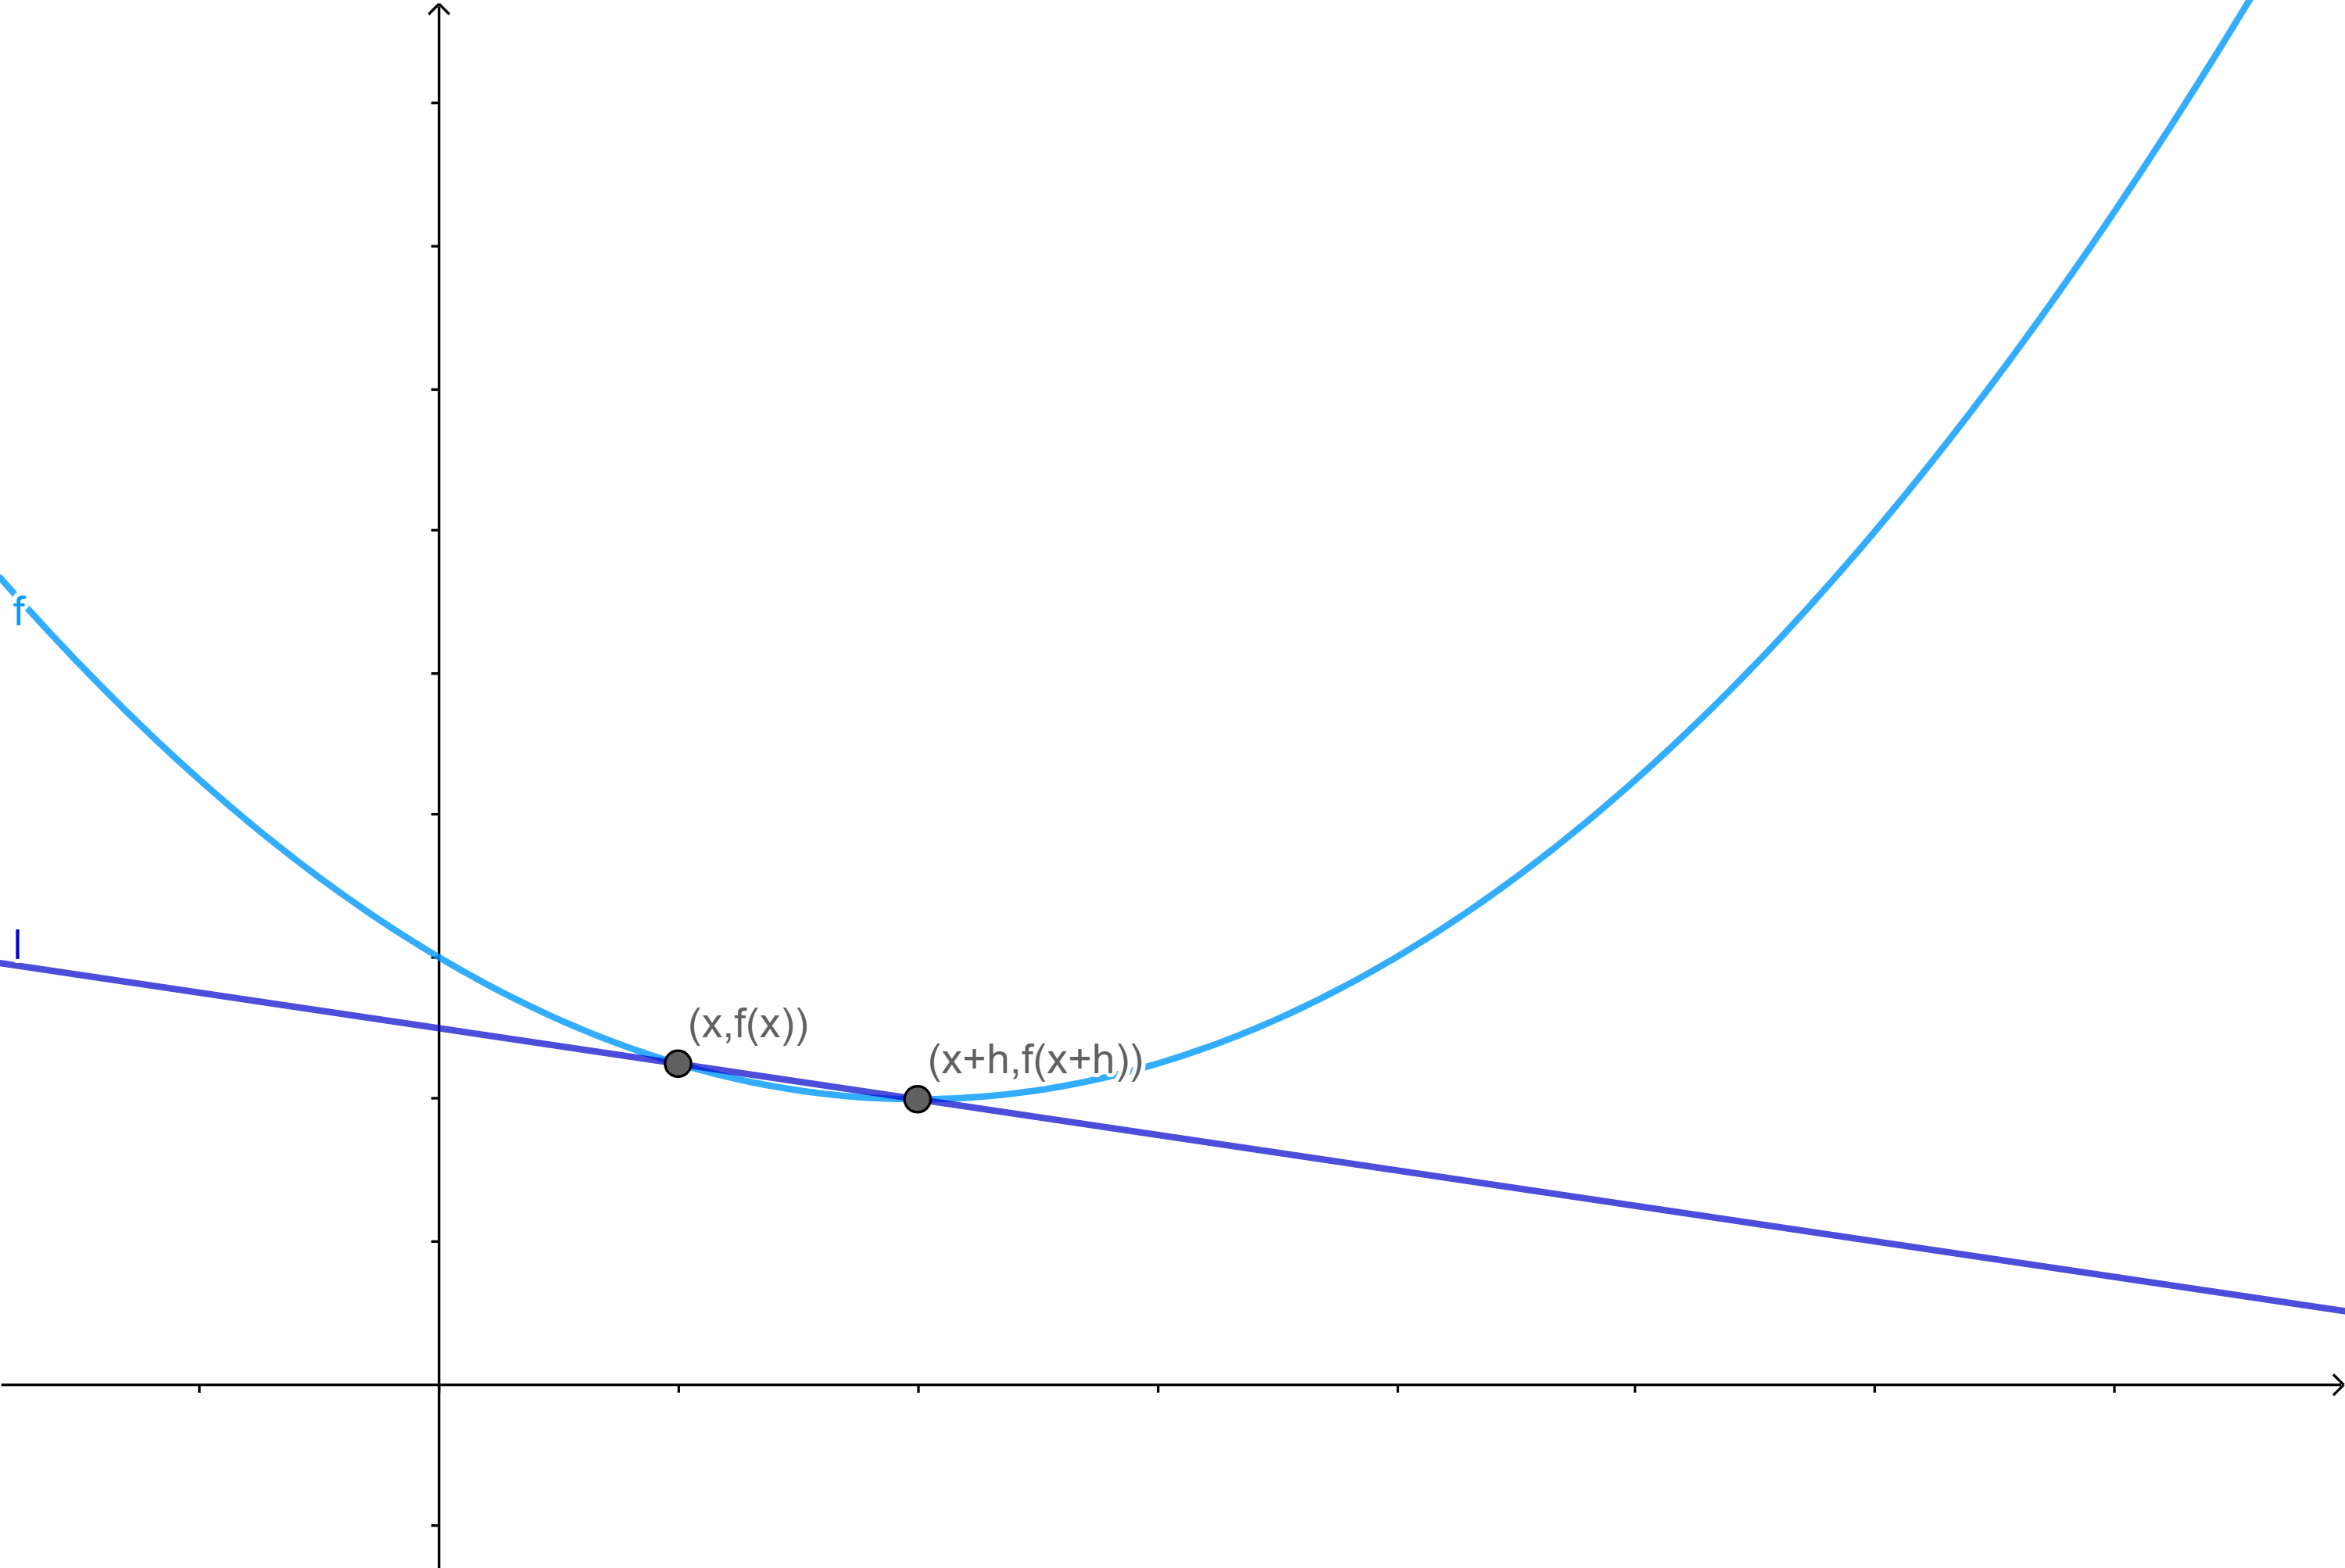
\includegraphics[width = 8cm]{Billeder/sekant2.png}
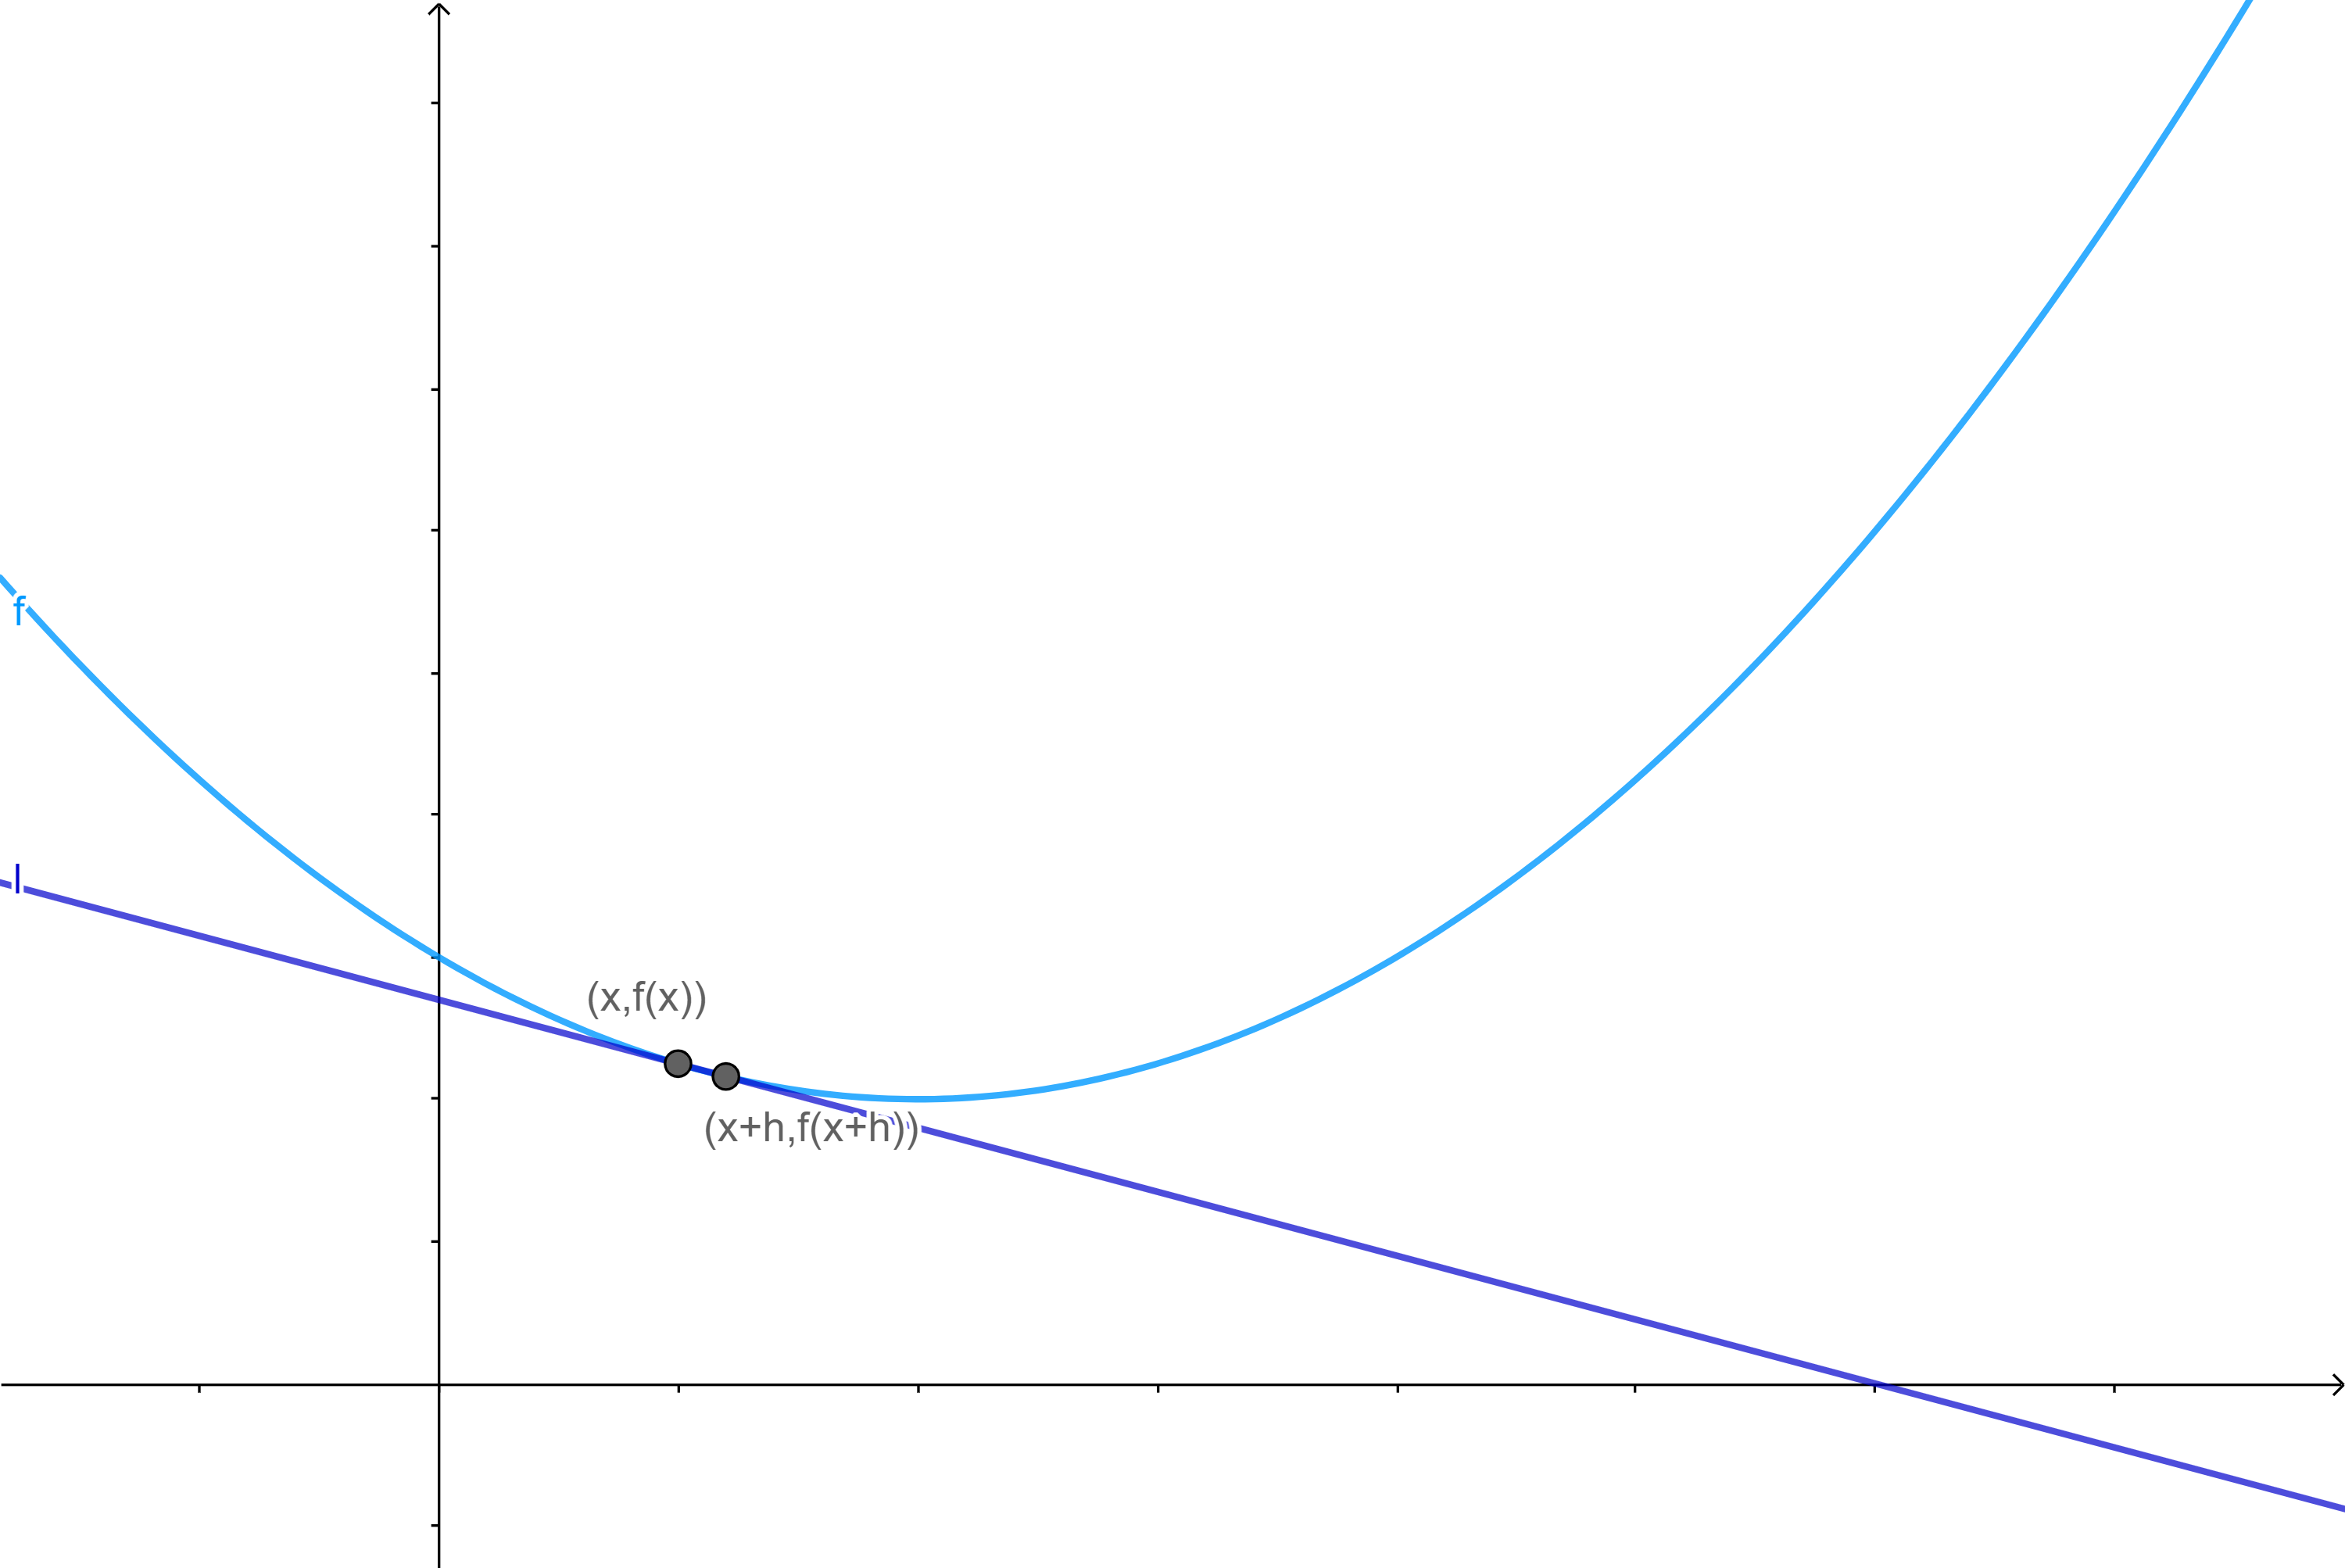
\includegraphics[width = 8cm]{Billeder/sekant3.png}
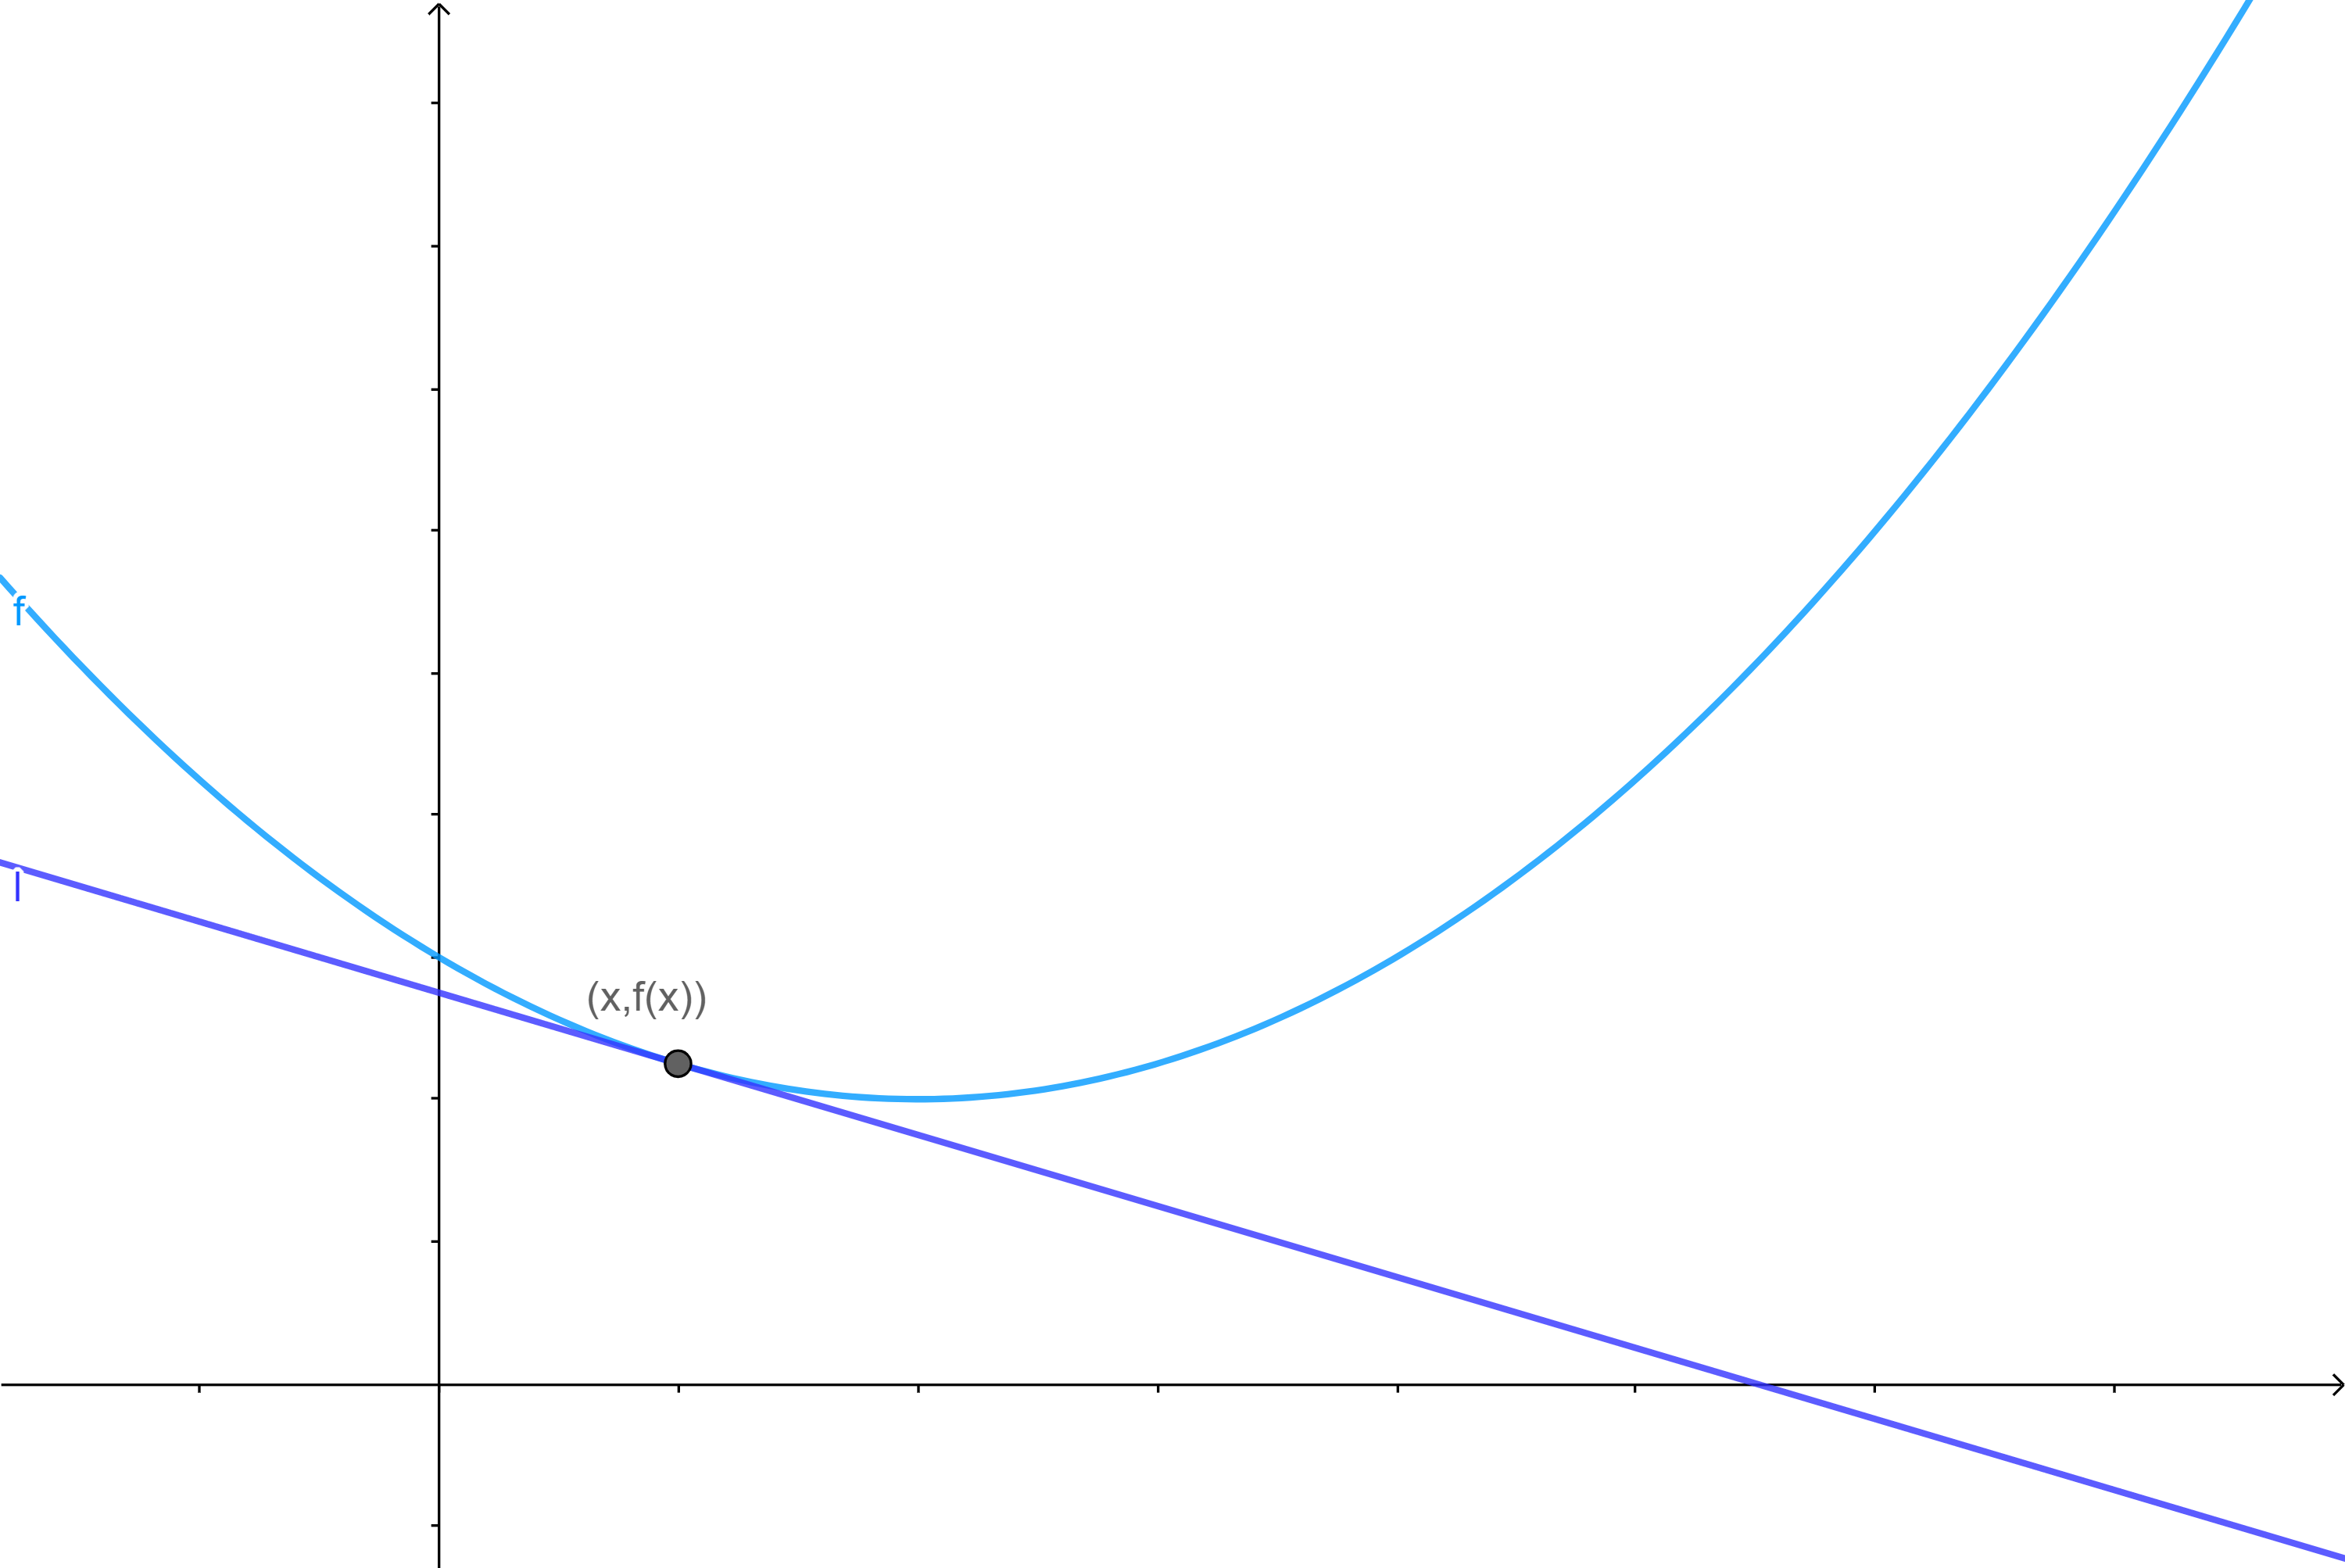
\includegraphics[width=8cm]{Billeder/tangent1.png}
\caption{Sekanterne gennem punkterne $(x_0,f(x_0))$ og $(x_0+h,f(x_0+h))$, når vi mindsker $h$. }
\label{fig:sek2}
\end{figure}
Det er hældningen af tangenten, vi har interesse i. Hældningen af sekanterne fra Fig. \ref{fig:sek1} og Fig. \ref{fig:sek2} er givet ved
\begin{align*}
\frac{f(x_0+h)-f(x)}{x_0+h-x_0} = \frac{f(x_0+h)-f(x_0)}{h}.
\end{align*}
Denne kaldes for differenskvotienten. Vi vil bestemme grænseværdien af differenskvotienten, når $h$ går mod $0$. Dette betegner vi med $\lim_{h\to 0}$, hvilket leder os til følgende definition:
\begin{defn}
Hvis grænsen 
\begin{align*}
\lim_{h\to 0} \frac{f(x_0+h)-f(x_0)}{h}
\end{align*}
eksisterer, så siger vi, at funktionen $f$ er differentiabel i $x_0$. Ydermere, så kalder vi grænseværdien 
\begin{align*}
f'(x_0) = \lim_{h\to 0} \frac{f(x_0+h)-f(x_0)}{h}
\end{align*}
for differentialkvotienten af $f$ i punktet $x_0$. Hvis denne eksisterer for alle $x$, så betragter vi $f'(x)$ som den afledede funktion af $f$. 
\end{defn}
Vi vil ikke komme mere ind på, hvad det specifikt betyder, at en grænseværdi eksisterer, men løst sagt går det ud på, at grænsen går mod et bestemt tal og ikke divergerer. 
differentialkvotienten kaldes også for den afledede af $f$ eller $f$-mærke. 

Vi vil nu lave vores første bevis:
\begin{setn}
	Funktionen $f$ givet ved
	\begin{align*}
		f(x) = x^2
	\end{align*}
	er differentiabel og har differentialkvotienten
	\begin{align*}
		f'(x) = 2x.
	\end{align*}
\end{setn}
\begin{proof}
	Vi indsætter vores funktion i definitionen for differentialkvotienten og vælger vores $x_0$ vilkårligt.
	\begin{align*}
		f'(x_0) &= \lim_{h\to 0}\frac{f(x_0 + h)-f(x_0)}{h}\\
		&=\lim_{h\to 0} \frac{(x_0+h)^2-x_0^2}{h}\\
		&=\lim_{h\to 0}\frac{x_0^2+h^2+2x_0h - x_0^2}{h}\\
		&=\lim_{h\to 0}\frac{h^2 + 2x_0h}{h}\\
		&= \lim_{h\to 0}h + 2x_0\\
		&=2x_0
	\end{align*}
	Da denne grænseværdi gælder for et vilkårligt $x_0$, så kan vi betragte $f'(x)$ som værende lig
	\begin{align*}
		f'(x) = 2x.
	\end{align*}
\end{proof}
\subsection*{Opgave 1}
\begin{enumerate}[label=\roman*)]
	\item Brug definitionen på differentialkvotienten til at bevise, at hvis 
	\begin{align*}
		f(x) = x,
	\end{align*}
	så er
	\begin{align*}
		f'(x) = 1
	\end{align*}	 
	\item Brug definitionen på differentialkvotienten til at bevise, at hvis 
	\begin{align*}
		f(x) = ax + b,
	\end{align*}		
	så er 
	\begin{align*}
		f'(x) = a.
	\end{align*}
	\item Brug definitionen på differentialkvotienten til at bevise, at hvis
	\begin{align*}
		f(x) = ax^2 + bx + c,
	\end{align*}	
	så er 
	\begin{align*}
		f'(x) = 	2ax + b.
	\end{align*}		
	\item Brug definitionen på differentialkvotienten til at bevise, at hvis
	\begin{align*}
		f(x) = k,
	\end{align*}
	så er 
	\begin{align*}
		f'(x) = 0
	\end{align*}
	\item Brug definitionen på differentialkvotienten til at bevise, at hvis
	\begin{align*}
		f(x) = x^3
	\end{align*}
	så er 
	\begin{align*}
		f'(x) = 3x^2.
	\end{align*}
\end{enumerate}